% The Loschmidt echo as a tensor network and, in the continuum, as a strip.
% Conventions follow carignano_tagliacozzo2025 (Fig. 9): filled circles for tensors, open circles
% for the product state, cream bands for the imaginary-time cooling, one boxed row for a Trotter
% layer and one boxed column for the transfer matrix.
%
% Standalone: compiles to imgs/echo_strip.pdf.
% Inline:     with \usepackage{standalone}, % The Loschmidt echo as a tensor network and, in the continuum, as a strip.
% Conventions follow carignano_tagliacozzo2025 (Fig. 9): filled circles for tensors, open circles
% for the product state, cream bands for the imaginary-time cooling, one boxed row for a Trotter
% layer and one boxed column for the transfer matrix.
%
% Standalone: compiles to imgs/echo_strip.pdf.
% Inline:     with \usepackage{standalone}, % The Loschmidt echo as a tensor network and, in the continuum, as a strip.
% Conventions follow carignano_tagliacozzo2025 (Fig. 9): filled circles for tensors, open circles
% for the product state, cream bands for the imaginary-time cooling, one boxed row for a Trotter
% layer and one boxed column for the transfer matrix.
%
% Standalone: compiles to imgs/echo_strip.pdf.
% Inline:     with \usepackage{standalone}, % The Loschmidt echo as a tensor network and, in the continuum, as a strip.
% Conventions follow carignano_tagliacozzo2025 (Fig. 9): filled circles for tensors, open circles
% for the product state, cream bands for the imaginary-time cooling, one boxed row for a Trotter
% layer and one boxed column for the transfer matrix.
%
% Standalone: compiles to imgs/echo_strip.pdf.
% Inline:     with \usepackage{standalone}, \input{imgs/echo_strip}.
\documentclass[tikz,border=3pt]{standalone}
\usepackage{amsmath,amssymb,braket}
\usetikzlibrary{arrows.meta,fadings}

\newcommand{\NX}{6}
\newcommand{\DX}{0.78}
\newcommand{\DY}{0.78}

\definecolor{tnbulk}{RGB}{86,196,229}
\definecolor{tncool}{RGB}{240,224,178}
\definecolor{tnbox}{RGB}{40,130,70}
\definecolor{tnrow}{RGB}{150,60,150}

\begin{document}
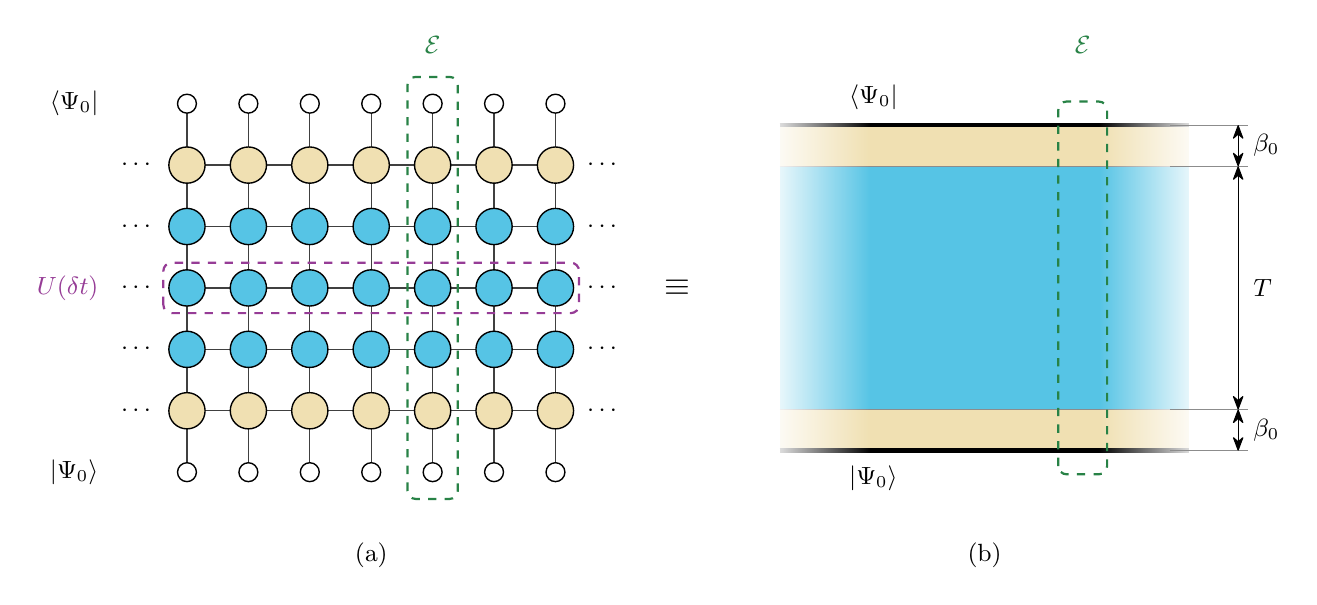
\begin{tikzpicture}[
    >={Stealth[round,length=2.0mm]},
    leg/.style={draw=black!75, line width=0.45pt},
    W/.style={circle, draw=black, fill=tnbulk, line width=0.5pt, minimum size=4.6mm, inner sep=0pt},
    B/.style={circle, draw=black, fill=tncool, line width=0.5pt, minimum size=4.6mm, inner sep=0pt},
    P/.style={circle, draw=black, fill=white, line width=0.5pt, minimum size=2.4mm, inner sep=0pt},
    vbox/.style={draw=tnbox, dashed, line width=0.8pt, rounded corners=3pt},
    hbox/.style={draw=tnrow, dashed, line width=0.8pt, rounded corners=3pt},
    tag/.style={font=\small},
  ]

  %% ================= panel (a): the lattice network =================
  \foreach \i in {0,...,\NX} { \draw[leg] (\i*\DX,0) -- (\i*\DX,{6*\DY}); }
  \foreach \j in {1,...,5} { \draw[leg] (0,\j*\DY) -- (\NX*\DX,\j*\DY); }

  \foreach \i in {0,...,\NX} {
    \foreach \j in {1,5} { \node[B] at (\i*\DX,\j*\DY) {}; }
    \foreach \j in {2,3,4} { \node[W] at (\i*\DX,\j*\DY) {}; }
    \node[P] at (\i*\DX,0)       {};
    \node[P] at (\i*\DX,{6*\DY}) {};
  }

  % the chain continues in both directions
  \foreach \j in {1,...,5} {
    \node[tag] at (-0.62,\j*\DY)             {$\cdots$};
    \node[tag] at ({\NX*\DX+0.62},\j*\DY)    {$\cdots$};
  }

  % one Trotter layer, and one spatial column
  \draw[hbox] (-0.30,{3*\DY-0.32}) rectangle ({\NX*\DX+0.30},{3*\DY+0.32});
  \node[tag, tnrow, anchor=east] at (-1.0,{3*\DY}) {$U(\delta t)$};
  \draw[vbox] ({4*\DX-0.32},-0.34) rectangle ({4*\DX+0.32},{6*\DY+0.34});
  \node[tag, tnbox] at ({4*\DX},{6*\DY+0.74}) {$\mathcal{E}$};

  \node[tag, anchor=east] at (-1.0,{6*\DY}) {$\bra{\Psi_0}$};
  \node[tag, anchor=east] at (-1.0,0)       {$\ket{\Psi_0}$};

  \node[tag] at ({\NX*\DX/2},-1.05) {(a)};

  \node[font=\large] at ({\NX*\DX+1.55},{3*\DY}) {$\equiv$};

  %% ================= panel (b): the continuum strip =================
  \begin{scope}[xshift={(\NX*\DX+2.85)*1cm}]
    \def\SW{5.2}
    \def\YA{0.35} \def\YB{1.02} \def\YC{4.98} \def\YD{5.65}

    \fill[tncool] (0,{\YA*\DY}) rectangle (\SW,{\YB*\DY});
    \fill[tnbulk] (0,{\YB*\DY}) rectangle (\SW,{\YC*\DY});
    \fill[tncool] (0,{\YC*\DY}) rectangle (\SW,{\YD*\DY});

    % the two edges are where the product state closes the path integral
    \draw[black, line width=1.6pt] (0,{\YA*\DY}) -- (\SW,{\YA*\DY});
    \draw[black, line width=1.6pt] (0,{\YD*\DY}) -- (\SW,{\YD*\DY});
    \draw[black!45, line width=0.4pt] (0,{\YB*\DY}) -- (\SW,{\YB*\DY});
    \draw[black!45, line width=0.4pt] (0,{\YC*\DY}) -- (\SW,{\YC*\DY});

    % fade both ends: the strip is infinite in the spatial direction
    \fill[white, path fading=east] (-0.18,{\YA*\DY-0.12}) rectangle (1.15,{\YD*\DY+0.12});
    \fill[white, path fading=west] ({\SW-1.15},{\YA*\DY-0.12}) rectangle ({\SW+0.18},{\YD*\DY+0.12});

    \node[tag, anchor=south east] at (1.62,{\YD*\DY+0.07}) {$\bra{\Psi_0}$};
    \node[tag, anchor=north east] at (1.62,{\YA*\DY-0.07}) {$\ket{\Psi_0}$};

    % guide lines are drawn after the fade so the dimensions stay legible
    \def\XD{\SW+0.62}
    \foreach \y in {\YA,\YB,\YC,\YD} {
      \draw[black!45, line width=0.35pt] ({\SW-0.25},{\y*\DY}) -- ({\XD+0.12},{\y*\DY});
    }
    \draw[<->] ({\XD},{\YB*\DY}) -- ({\XD},{\YC*\DY}) node[midway, right=2pt, tag] {$T$};
    \draw[<->] ({\XD},{\YA*\DY}) -- ({\XD},{\YB*\DY}) node[midway, right=2pt, tag] {$\beta_0$};
    \draw[<->] ({\XD},{\YC*\DY}) -- ({\XD},{\YD*\DY}) node[midway, right=2pt, tag] {$\beta_0$};

    \draw[vbox] ({0.68*\SW},{\YA*\DY-0.30}) rectangle ({0.68*\SW+0.62},{\YD*\DY+0.30});
    \node[tag, tnbox] at ({0.68*\SW+0.31},{6*\DY+0.74}) {$\mathcal{E}$};

    \node[tag] at ({\SW/2},-1.05) {(b)};
  \end{scope}

\end{tikzpicture}
\end{document}
.
\documentclass[tikz,border=3pt]{standalone}
\usepackage{amsmath,amssymb,braket}
\usetikzlibrary{arrows.meta,fadings}

\newcommand{\NX}{6}
\newcommand{\DX}{0.78}
\newcommand{\DY}{0.78}

\definecolor{tnbulk}{RGB}{86,196,229}
\definecolor{tncool}{RGB}{240,224,178}
\definecolor{tnbox}{RGB}{40,130,70}
\definecolor{tnrow}{RGB}{150,60,150}

\begin{document}
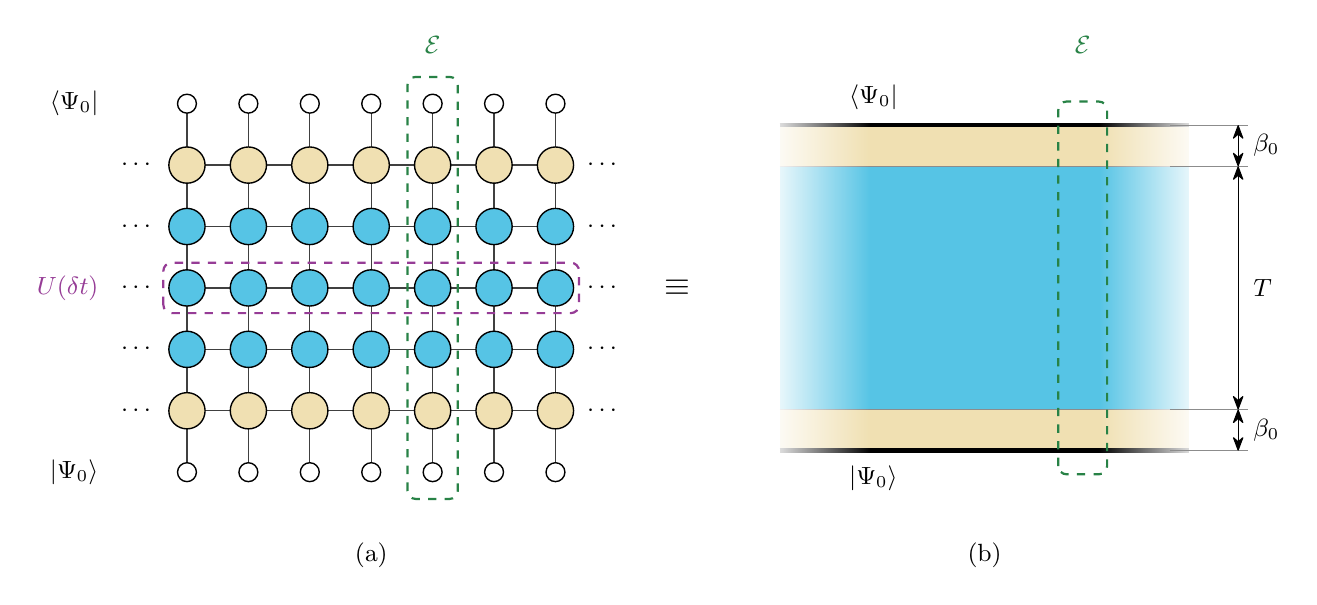
\begin{tikzpicture}[
    >={Stealth[round,length=2.0mm]},
    leg/.style={draw=black!75, line width=0.45pt},
    W/.style={circle, draw=black, fill=tnbulk, line width=0.5pt, minimum size=4.6mm, inner sep=0pt},
    B/.style={circle, draw=black, fill=tncool, line width=0.5pt, minimum size=4.6mm, inner sep=0pt},
    P/.style={circle, draw=black, fill=white, line width=0.5pt, minimum size=2.4mm, inner sep=0pt},
    vbox/.style={draw=tnbox, dashed, line width=0.8pt, rounded corners=3pt},
    hbox/.style={draw=tnrow, dashed, line width=0.8pt, rounded corners=3pt},
    tag/.style={font=\small},
  ]

  %% ================= panel (a): the lattice network =================
  \foreach \i in {0,...,\NX} { \draw[leg] (\i*\DX,0) -- (\i*\DX,{6*\DY}); }
  \foreach \j in {1,...,5} { \draw[leg] (0,\j*\DY) -- (\NX*\DX,\j*\DY); }

  \foreach \i in {0,...,\NX} {
    \foreach \j in {1,5} { \node[B] at (\i*\DX,\j*\DY) {}; }
    \foreach \j in {2,3,4} { \node[W] at (\i*\DX,\j*\DY) {}; }
    \node[P] at (\i*\DX,0)       {};
    \node[P] at (\i*\DX,{6*\DY}) {};
  }

  % the chain continues in both directions
  \foreach \j in {1,...,5} {
    \node[tag] at (-0.62,\j*\DY)             {$\cdots$};
    \node[tag] at ({\NX*\DX+0.62},\j*\DY)    {$\cdots$};
  }

  % one Trotter layer, and one spatial column
  \draw[hbox] (-0.30,{3*\DY-0.32}) rectangle ({\NX*\DX+0.30},{3*\DY+0.32});
  \node[tag, tnrow, anchor=east] at (-1.0,{3*\DY}) {$U(\delta t)$};
  \draw[vbox] ({4*\DX-0.32},-0.34) rectangle ({4*\DX+0.32},{6*\DY+0.34});
  \node[tag, tnbox] at ({4*\DX},{6*\DY+0.74}) {$\mathcal{E}$};

  \node[tag, anchor=east] at (-1.0,{6*\DY}) {$\bra{\Psi_0}$};
  \node[tag, anchor=east] at (-1.0,0)       {$\ket{\Psi_0}$};

  \node[tag] at ({\NX*\DX/2},-1.05) {(a)};

  \node[font=\large] at ({\NX*\DX+1.55},{3*\DY}) {$\equiv$};

  %% ================= panel (b): the continuum strip =================
  \begin{scope}[xshift={(\NX*\DX+2.85)*1cm}]
    \def\SW{5.2}
    \def\YA{0.35} \def\YB{1.02} \def\YC{4.98} \def\YD{5.65}

    \fill[tncool] (0,{\YA*\DY}) rectangle (\SW,{\YB*\DY});
    \fill[tnbulk] (0,{\YB*\DY}) rectangle (\SW,{\YC*\DY});
    \fill[tncool] (0,{\YC*\DY}) rectangle (\SW,{\YD*\DY});

    % the two edges are where the product state closes the path integral
    \draw[black, line width=1.6pt] (0,{\YA*\DY}) -- (\SW,{\YA*\DY});
    \draw[black, line width=1.6pt] (0,{\YD*\DY}) -- (\SW,{\YD*\DY});
    \draw[black!45, line width=0.4pt] (0,{\YB*\DY}) -- (\SW,{\YB*\DY});
    \draw[black!45, line width=0.4pt] (0,{\YC*\DY}) -- (\SW,{\YC*\DY});

    % fade both ends: the strip is infinite in the spatial direction
    \fill[white, path fading=east] (-0.18,{\YA*\DY-0.12}) rectangle (1.15,{\YD*\DY+0.12});
    \fill[white, path fading=west] ({\SW-1.15},{\YA*\DY-0.12}) rectangle ({\SW+0.18},{\YD*\DY+0.12});

    \node[tag, anchor=south east] at (1.62,{\YD*\DY+0.07}) {$\bra{\Psi_0}$};
    \node[tag, anchor=north east] at (1.62,{\YA*\DY-0.07}) {$\ket{\Psi_0}$};

    % guide lines are drawn after the fade so the dimensions stay legible
    \def\XD{\SW+0.62}
    \foreach \y in {\YA,\YB,\YC,\YD} {
      \draw[black!45, line width=0.35pt] ({\SW-0.25},{\y*\DY}) -- ({\XD+0.12},{\y*\DY});
    }
    \draw[<->] ({\XD},{\YB*\DY}) -- ({\XD},{\YC*\DY}) node[midway, right=2pt, tag] {$T$};
    \draw[<->] ({\XD},{\YA*\DY}) -- ({\XD},{\YB*\DY}) node[midway, right=2pt, tag] {$\beta_0$};
    \draw[<->] ({\XD},{\YC*\DY}) -- ({\XD},{\YD*\DY}) node[midway, right=2pt, tag] {$\beta_0$};

    \draw[vbox] ({0.68*\SW},{\YA*\DY-0.30}) rectangle ({0.68*\SW+0.62},{\YD*\DY+0.30});
    \node[tag, tnbox] at ({0.68*\SW+0.31},{6*\DY+0.74}) {$\mathcal{E}$};

    \node[tag] at ({\SW/2},-1.05) {(b)};
  \end{scope}

\end{tikzpicture}
\end{document}
.
\documentclass[tikz,border=3pt]{standalone}
\usepackage{amsmath,amssymb,braket}
\usetikzlibrary{arrows.meta,fadings}

\newcommand{\NX}{6}
\newcommand{\DX}{0.78}
\newcommand{\DY}{0.78}

\definecolor{tnbulk}{RGB}{86,196,229}
\definecolor{tncool}{RGB}{240,224,178}
\definecolor{tnbox}{RGB}{40,130,70}
\definecolor{tnrow}{RGB}{150,60,150}

\begin{document}
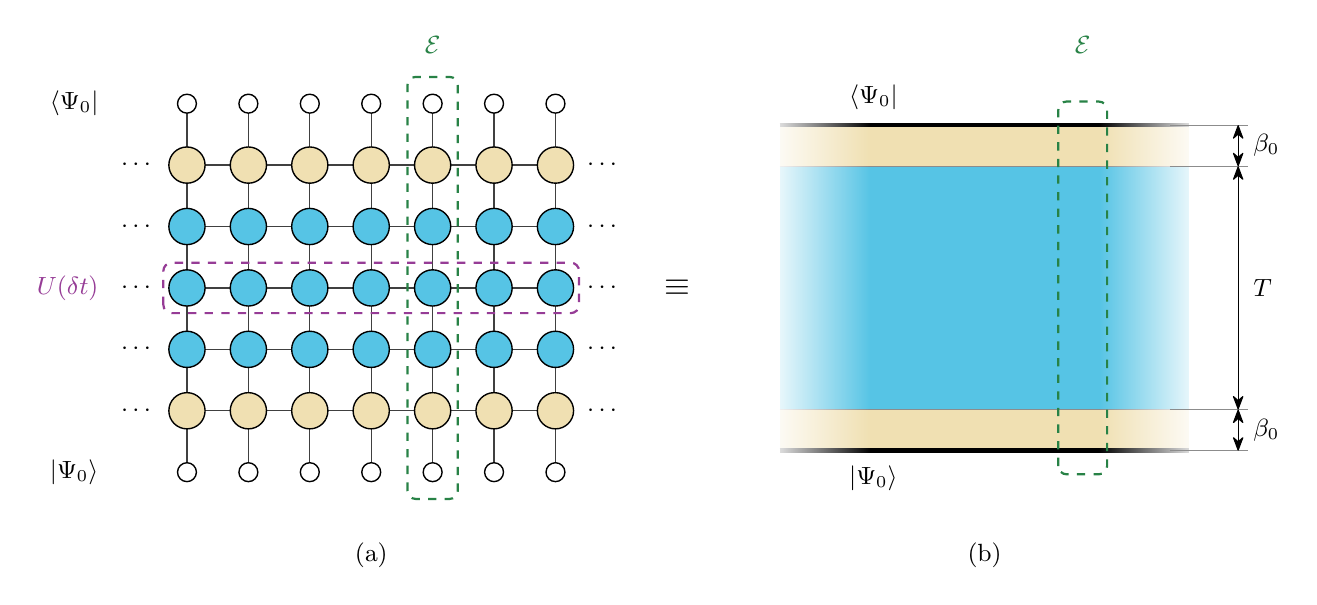
\begin{tikzpicture}[
    >={Stealth[round,length=2.0mm]},
    leg/.style={draw=black!75, line width=0.45pt},
    W/.style={circle, draw=black, fill=tnbulk, line width=0.5pt, minimum size=4.6mm, inner sep=0pt},
    B/.style={circle, draw=black, fill=tncool, line width=0.5pt, minimum size=4.6mm, inner sep=0pt},
    P/.style={circle, draw=black, fill=white, line width=0.5pt, minimum size=2.4mm, inner sep=0pt},
    vbox/.style={draw=tnbox, dashed, line width=0.8pt, rounded corners=3pt},
    hbox/.style={draw=tnrow, dashed, line width=0.8pt, rounded corners=3pt},
    tag/.style={font=\small},
  ]

  %% ================= panel (a): the lattice network =================
  \foreach \i in {0,...,\NX} { \draw[leg] (\i*\DX,0) -- (\i*\DX,{6*\DY}); }
  \foreach \j in {1,...,5} { \draw[leg] (0,\j*\DY) -- (\NX*\DX,\j*\DY); }

  \foreach \i in {0,...,\NX} {
    \foreach \j in {1,5} { \node[B] at (\i*\DX,\j*\DY) {}; }
    \foreach \j in {2,3,4} { \node[W] at (\i*\DX,\j*\DY) {}; }
    \node[P] at (\i*\DX,0)       {};
    \node[P] at (\i*\DX,{6*\DY}) {};
  }

  % the chain continues in both directions
  \foreach \j in {1,...,5} {
    \node[tag] at (-0.62,\j*\DY)             {$\cdots$};
    \node[tag] at ({\NX*\DX+0.62},\j*\DY)    {$\cdots$};
  }

  % one Trotter layer, and one spatial column
  \draw[hbox] (-0.30,{3*\DY-0.32}) rectangle ({\NX*\DX+0.30},{3*\DY+0.32});
  \node[tag, tnrow, anchor=east] at (-1.0,{3*\DY}) {$U(\delta t)$};
  \draw[vbox] ({4*\DX-0.32},-0.34) rectangle ({4*\DX+0.32},{6*\DY+0.34});
  \node[tag, tnbox] at ({4*\DX},{6*\DY+0.74}) {$\mathcal{E}$};

  \node[tag, anchor=east] at (-1.0,{6*\DY}) {$\bra{\Psi_0}$};
  \node[tag, anchor=east] at (-1.0,0)       {$\ket{\Psi_0}$};

  \node[tag] at ({\NX*\DX/2},-1.05) {(a)};

  \node[font=\large] at ({\NX*\DX+1.55},{3*\DY}) {$\equiv$};

  %% ================= panel (b): the continuum strip =================
  \begin{scope}[xshift={(\NX*\DX+2.85)*1cm}]
    \def\SW{5.2}
    \def\YA{0.35} \def\YB{1.02} \def\YC{4.98} \def\YD{5.65}

    \fill[tncool] (0,{\YA*\DY}) rectangle (\SW,{\YB*\DY});
    \fill[tnbulk] (0,{\YB*\DY}) rectangle (\SW,{\YC*\DY});
    \fill[tncool] (0,{\YC*\DY}) rectangle (\SW,{\YD*\DY});

    % the two edges are where the product state closes the path integral
    \draw[black, line width=1.6pt] (0,{\YA*\DY}) -- (\SW,{\YA*\DY});
    \draw[black, line width=1.6pt] (0,{\YD*\DY}) -- (\SW,{\YD*\DY});
    \draw[black!45, line width=0.4pt] (0,{\YB*\DY}) -- (\SW,{\YB*\DY});
    \draw[black!45, line width=0.4pt] (0,{\YC*\DY}) -- (\SW,{\YC*\DY});

    % fade both ends: the strip is infinite in the spatial direction
    \fill[white, path fading=east] (-0.18,{\YA*\DY-0.12}) rectangle (1.15,{\YD*\DY+0.12});
    \fill[white, path fading=west] ({\SW-1.15},{\YA*\DY-0.12}) rectangle ({\SW+0.18},{\YD*\DY+0.12});

    \node[tag, anchor=south east] at (1.62,{\YD*\DY+0.07}) {$\bra{\Psi_0}$};
    \node[tag, anchor=north east] at (1.62,{\YA*\DY-0.07}) {$\ket{\Psi_0}$};

    % guide lines are drawn after the fade so the dimensions stay legible
    \def\XD{\SW+0.62}
    \foreach \y in {\YA,\YB,\YC,\YD} {
      \draw[black!45, line width=0.35pt] ({\SW-0.25},{\y*\DY}) -- ({\XD+0.12},{\y*\DY});
    }
    \draw[<->] ({\XD},{\YB*\DY}) -- ({\XD},{\YC*\DY}) node[midway, right=2pt, tag] {$T$};
    \draw[<->] ({\XD},{\YA*\DY}) -- ({\XD},{\YB*\DY}) node[midway, right=2pt, tag] {$\beta_0$};
    \draw[<->] ({\XD},{\YC*\DY}) -- ({\XD},{\YD*\DY}) node[midway, right=2pt, tag] {$\beta_0$};

    \draw[vbox] ({0.68*\SW},{\YA*\DY-0.30}) rectangle ({0.68*\SW+0.62},{\YD*\DY+0.30});
    \node[tag, tnbox] at ({0.68*\SW+0.31},{6*\DY+0.74}) {$\mathcal{E}$};

    \node[tag] at ({\SW/2},-1.05) {(b)};
  \end{scope}

\end{tikzpicture}
\end{document}
.
\documentclass[tikz,border=3pt]{standalone}
\usepackage{amsmath,amssymb,braket}
\usetikzlibrary{arrows.meta,fadings}

\newcommand{\NX}{6}
\newcommand{\DX}{0.78}
\newcommand{\DY}{0.78}

\definecolor{tnbulk}{RGB}{86,196,229}
\definecolor{tncool}{RGB}{240,224,178}
\definecolor{tnbox}{RGB}{40,130,70}
\definecolor{tnrow}{RGB}{150,60,150}

\begin{document}
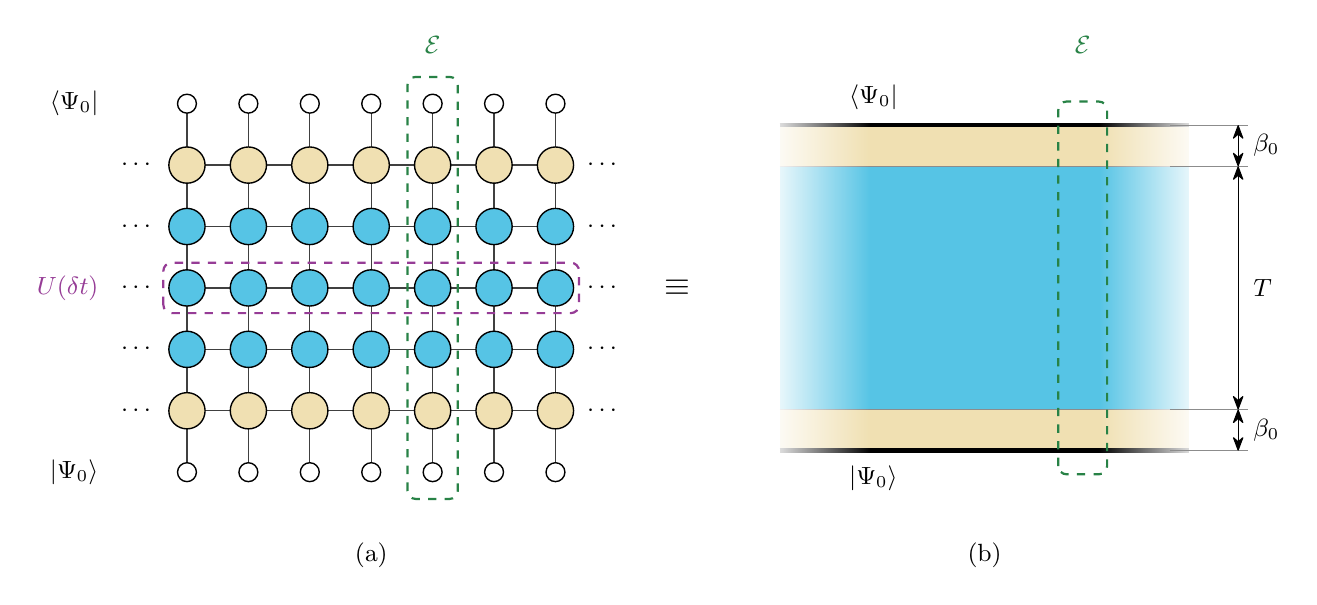
\begin{tikzpicture}[
    >={Stealth[round,length=2.0mm]},
    leg/.style={draw=black!75, line width=0.45pt},
    W/.style={circle, draw=black, fill=tnbulk, line width=0.5pt, minimum size=4.6mm, inner sep=0pt},
    B/.style={circle, draw=black, fill=tncool, line width=0.5pt, minimum size=4.6mm, inner sep=0pt},
    P/.style={circle, draw=black, fill=white, line width=0.5pt, minimum size=2.4mm, inner sep=0pt},
    vbox/.style={draw=tnbox, dashed, line width=0.8pt, rounded corners=3pt},
    hbox/.style={draw=tnrow, dashed, line width=0.8pt, rounded corners=3pt},
    tag/.style={font=\small},
  ]

  %% ================= panel (a): the lattice network =================
  \foreach \i in {0,...,\NX} { \draw[leg] (\i*\DX,0) -- (\i*\DX,{6*\DY}); }
  \foreach \j in {1,...,5} { \draw[leg] (0,\j*\DY) -- (\NX*\DX,\j*\DY); }

  \foreach \i in {0,...,\NX} {
    \foreach \j in {1,5} { \node[B] at (\i*\DX,\j*\DY) {}; }
    \foreach \j in {2,3,4} { \node[W] at (\i*\DX,\j*\DY) {}; }
    \node[P] at (\i*\DX,0)       {};
    \node[P] at (\i*\DX,{6*\DY}) {};
  }

  % the chain continues in both directions
  \foreach \j in {1,...,5} {
    \node[tag] at (-0.62,\j*\DY)             {$\cdots$};
    \node[tag] at ({\NX*\DX+0.62},\j*\DY)    {$\cdots$};
  }

  % one Trotter layer, and one spatial column
  \draw[hbox] (-0.30,{3*\DY-0.32}) rectangle ({\NX*\DX+0.30},{3*\DY+0.32});
  \node[tag, tnrow, anchor=east] at (-1.0,{3*\DY}) {$U(\delta t)$};
  \draw[vbox] ({4*\DX-0.32},-0.34) rectangle ({4*\DX+0.32},{6*\DY+0.34});
  \node[tag, tnbox] at ({4*\DX},{6*\DY+0.74}) {$\mathcal{E}$};

  \node[tag, anchor=east] at (-1.0,{6*\DY}) {$\bra{\Psi_0}$};
  \node[tag, anchor=east] at (-1.0,0)       {$\ket{\Psi_0}$};

  \node[tag] at ({\NX*\DX/2},-1.05) {(a)};

  \node[font=\large] at ({\NX*\DX+1.55},{3*\DY}) {$\equiv$};

  %% ================= panel (b): the continuum strip =================
  \begin{scope}[xshift={(\NX*\DX+2.85)*1cm}]
    \def\SW{5.2}
    \def\YA{0.35} \def\YB{1.02} \def\YC{4.98} \def\YD{5.65}

    \fill[tncool] (0,{\YA*\DY}) rectangle (\SW,{\YB*\DY});
    \fill[tnbulk] (0,{\YB*\DY}) rectangle (\SW,{\YC*\DY});
    \fill[tncool] (0,{\YC*\DY}) rectangle (\SW,{\YD*\DY});

    % the two edges are where the product state closes the path integral
    \draw[black, line width=1.6pt] (0,{\YA*\DY}) -- (\SW,{\YA*\DY});
    \draw[black, line width=1.6pt] (0,{\YD*\DY}) -- (\SW,{\YD*\DY});
    \draw[black!45, line width=0.4pt] (0,{\YB*\DY}) -- (\SW,{\YB*\DY});
    \draw[black!45, line width=0.4pt] (0,{\YC*\DY}) -- (\SW,{\YC*\DY});

    % fade both ends: the strip is infinite in the spatial direction
    \fill[white, path fading=east] (-0.18,{\YA*\DY-0.12}) rectangle (1.15,{\YD*\DY+0.12});
    \fill[white, path fading=west] ({\SW-1.15},{\YA*\DY-0.12}) rectangle ({\SW+0.18},{\YD*\DY+0.12});

    \node[tag, anchor=south east] at (1.62,{\YD*\DY+0.07}) {$\bra{\Psi_0}$};
    \node[tag, anchor=north east] at (1.62,{\YA*\DY-0.07}) {$\ket{\Psi_0}$};

    % guide lines are drawn after the fade so the dimensions stay legible
    \def\XD{\SW+0.62}
    \foreach \y in {\YA,\YB,\YC,\YD} {
      \draw[black!45, line width=0.35pt] ({\SW-0.25},{\y*\DY}) -- ({\XD+0.12},{\y*\DY});
    }
    \draw[<->] ({\XD},{\YB*\DY}) -- ({\XD},{\YC*\DY}) node[midway, right=2pt, tag] {$T$};
    \draw[<->] ({\XD},{\YA*\DY}) -- ({\XD},{\YB*\DY}) node[midway, right=2pt, tag] {$\beta_0$};
    \draw[<->] ({\XD},{\YC*\DY}) -- ({\XD},{\YD*\DY}) node[midway, right=2pt, tag] {$\beta_0$};

    \draw[vbox] ({0.68*\SW},{\YA*\DY-0.30}) rectangle ({0.68*\SW+0.62},{\YD*\DY+0.30});
    \node[tag, tnbox] at ({0.68*\SW+0.31},{6*\DY+0.74}) {$\mathcal{E}$};

    \node[tag] at ({\SW/2},-1.05) {(b)};
  \end{scope}

\end{tikzpicture}
\end{document}
